%%%%%%%%%%%%%%%%%%%%%%%%%%%%%%%%%%%%%%%%%%%%%%%%%%%%%%%%%%%
% --------------------------------------------------------
% Rho
% LaTeX Template
% Version 2.0.0 (21/05/2024)
%
% Authors: 
% Guillermo Jimenez (memo.notess1@gmail.com)
% Eduardo Gracidas (eduardo.gracidas29@gmail.com)
% 
% License:
% Creative Commons CC BY 4.0
% --------------------------------------------------------
%%%%%%%%%%%%%%%%%%%%%%%%%%%%%%%%%%%%%%%%%%%%%%%%%%%%%%%%%%%

\documentclass[9pt,a4paper,twoside]{rho-class/rho}
\setbool{rho-abstract}{false} % Set false to hide the abstract
\setbool{corres-info}{false} % Set false to hide the corresponding author section
\setbool{linenumbers}{false} % Set false to hide the line numbering

%----------------------------------------------------------
% TITLE
%----------------------------------------------------------

\journalname{Processos Estocásticos e Vibrações Aleatórias}
\title{Trabalho}

%----------------------------------------------------------
% AUTHORS AND AFFILIATIONS
%----------------------------------------------------------

\author[1]{Leonardo Maia Nogueira}


%----------------------------------------------------------




%----------------------------------------------------------
% DATES
%----------------------------------------------------------

%\dates{This manuscript was compile on April 28, 2024}

%----------------------------------------------------------
% FOOTER INFORMATION
%----------------------------------------------------------

\leadauthor{Author last name et al.}
\footinfo{Creative Commons CC BY 4.0}
\smalltitle{\LaTeX\ Template}
\institution{College name}
\theday{May 21, 2024} %\today

%----------------------------------------------------------
% ARTICLE INFORMATION
%----------------------------------------------------------

\corres{Provide the corresponding author information and publisher here.}
\email{example@organization.com.}
\doi{\url{https://www.doi.org/exampledoi/XXXXXXXXXX}}

\received{March 20, 2024}
\revised{April 16, 2024}
\accepted{April 20, 2024}
\published{May 21, 2024}

\license{Rho LaTeX Class \ccLogo\ This document is licensed under Creative Commons CC BY 4.0.}

%----------------------------------------------------------
% ABSTRACT
%----------------------------------------------------------


%----------------------------------------------------------



%----------------------------------------------------------

\begin{document}
	
    \maketitle
    \thispagestyle{firststyle}
    % \tableofcontents

%----------------------------------------------------------

\section{Enunciado}
O artigo Hambric et al 2004, "Vibrations of plates with clamped and free edges excited by low-speed
turbulent boundary layer flow.", fornecido junto com o trabalho apresenta uma análise da resposta
vibratória de uma placa submetida a uma excitação na forma de uma camada limite turbulenta (TBL -
Turbulent Boundary Layer). O artigo examina diferentes condições de contorno para a placa e algumas
simplificações para o modelo de TBL empregado (modelo de Corcos).
\begin{figure}[H]
	\centering
	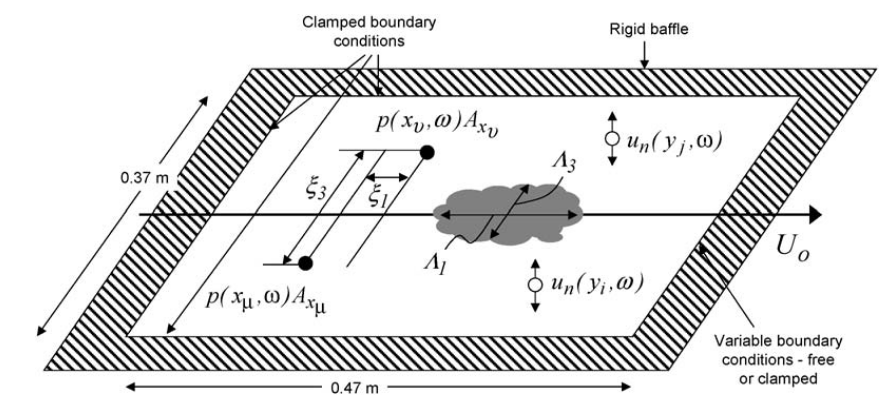
\includegraphics[width=0.9\columnwidth]{figures/schema_TBL.png}
	\caption{Esquemático do Artigo de Hambric}
	\label{fig:schmtbl}
\end{figure}

De forma similar, o artigo Marcheto et al 2017, "Vibroacoustic response of panels under diffuse acousticfield excitation from sensitivity functions and reciprocityprinciples" examina a resposta vibratória de um painel submetido a uma excitação aleatória distribuída na forma de um Campo Acústico Difuso. 
\begin{figure}[H]
	\centering
	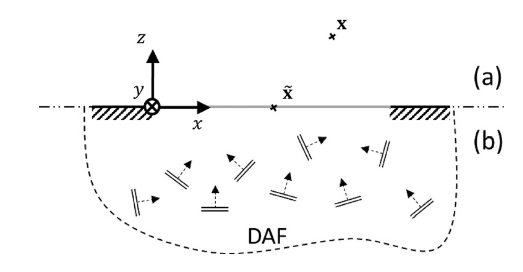
\includegraphics[width=0.9\columnwidth]{figures/schema_DAF.png}
	\caption{Esquemático do Artiho de Machetto}
	\label{fig:schmdaf}
\end{figure}


Com base nos artigos e utilizando o código em MatLab fornecido com um modelo de placa em FEM, faça:

\begin{enumerate}
	\item  Reproduza os resultados do artigo Hambric et al 2004 para a condição analisada com uma borda livre;
	\item Calcule a resposta da placa considerada no item 1, considerando uma excitação na forma de um campo acústico difuso. Para tanto, considere a formulação para a densidade espectral cruzada fornecida no artigo Marcheto et al 2017 e o Autoespectro encontrado no item 1.
	\item Compare as resposta e discuta os resultados.
\end{enumerate}

\section{Solução}
\subsection{Auto Espectro}
Segundo \cite{hambricVibrationsPlatesClamped2004}, o espectro cruzado da pressão acústica exercida por um escoamento turbulento paralelo a uma placa pode ser definido pela equação abaixo.
\begin{equation}
	\Phi_{pp}(x_\mu,x_v,\omega)=\bar{\phi}_{pp}(\omega)\Gamma(\xi_1,\xi_3,\omega),
\end{equation}
onde $\phi_{pp}$ é o auto espectro da pressão, que pode ser satisfatoriamente aproximado pela equação a seguir.
\begin{equation}
	\phi_{pp}(\omega)\approx\left(\frac{\tau_w^2\delta^*}{U_0}\right)\left(\frac{5.1}{1+0.44(\omega\delta^*/U_0)^{7/3}}\right)
\end{equation}

\begin{equation}
	\mathrm{Re}_\delta\approx8U_0\delta^*/\nu, \quad \tau_w\approx0.0225\rho U_0^2/\mathrm{Re}_\delta^{0.25}
\end{equation}
Calculando-se o auto espectro da pressão acústica para as velocidades de fluxo, como visto em Hambric \cite{hambricVibrationsPlatesClamped2004} podemos expressar graficamente estes resultados em função da frequência como visto na Figura~\ref{fig:psd}.
\begin{figure}[H]
	\centering
	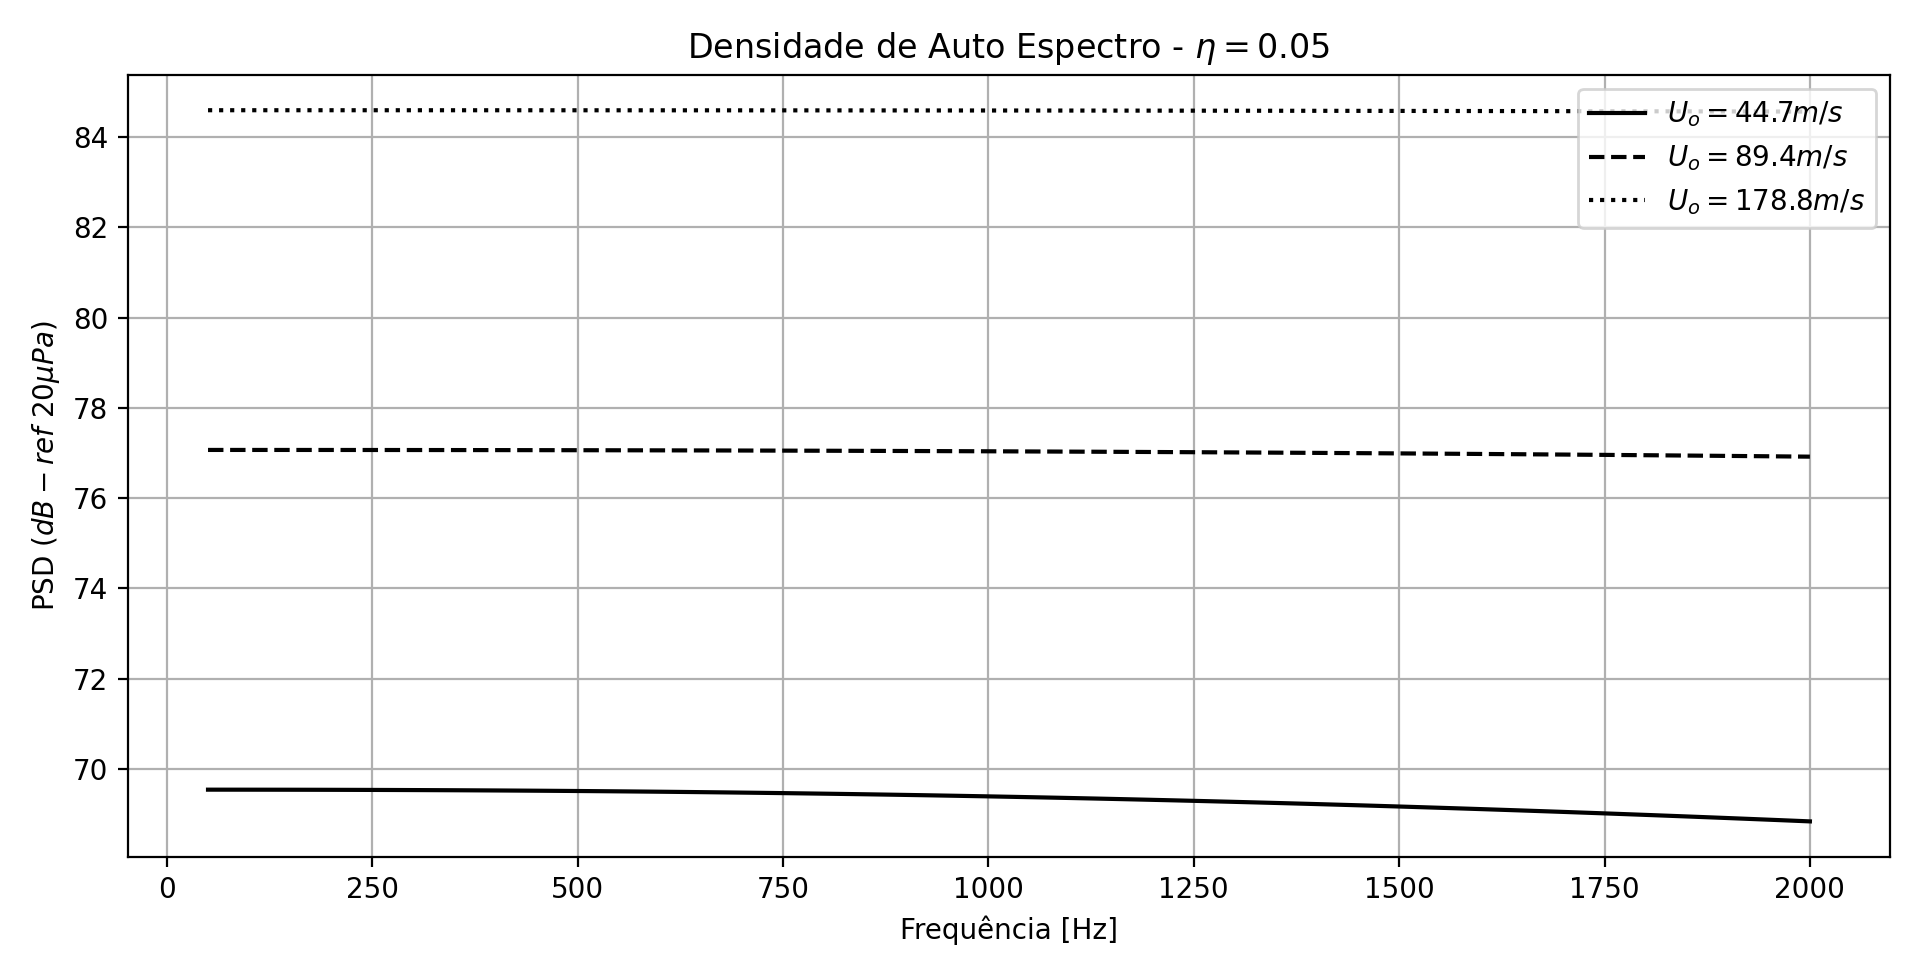
\includegraphics[width=0.9\columnwidth]{figures/psd_vel.png}
	\caption{Autoespectro de Entrada}
	\label{fig:psd}
\end{figure}
Não foi observada significante alteração do comportamento com a variação de amortecimento $\eta$.

\subsection{Coerência}

O próximo passo é encontrar o espectro da coerência $\Gamma(\xi_1,\xi_3,\omega)$ com as equações a seguir. 
\begin{equation}
	\Gamma(\xi_1,\xi_3,\omega)=A(\omega\xi_1/U_c)B(\omega\xi_3/U_c)
\end{equation}

\begin{equation}
	U_c\cong U_0(0.59+0.30\mathrm{e}^{-0.89\omega\delta^*/U_0})
\end{equation}

\begin{eqnarray}
	A(\omega\xi_1/U_c)=(1+\alpha_1|\omega\xi_1/U_c|)\mathrm{e}^{-\alpha_1|\omega\xi_1/U_c|}\mathrm{e}^{\mathrm{i}\omega\xi_1/U_c} \\
	B(\omega\xi_3/U_c)=\mathrm{e}^{-\alpha_3|\omega\xi_3/U_c|}
\end{eqnarray}
O artigo de Hambric~\cite{hambricVibrationsPlatesClamped2004} define como ponto de observação o ponto de coordenadas $(15cm, 12cm)$ a partir do vértice inferior a esquerda, que no caso do modelo em Elementos Finitos desenvolvido neste trabalho é o nó 227. A coerência do nó 701 em relação a todos os nós em função da frequência pode ser observado na Figura~\ref{fig:coerTBL}

\begin{figure}[H]
	\centering
	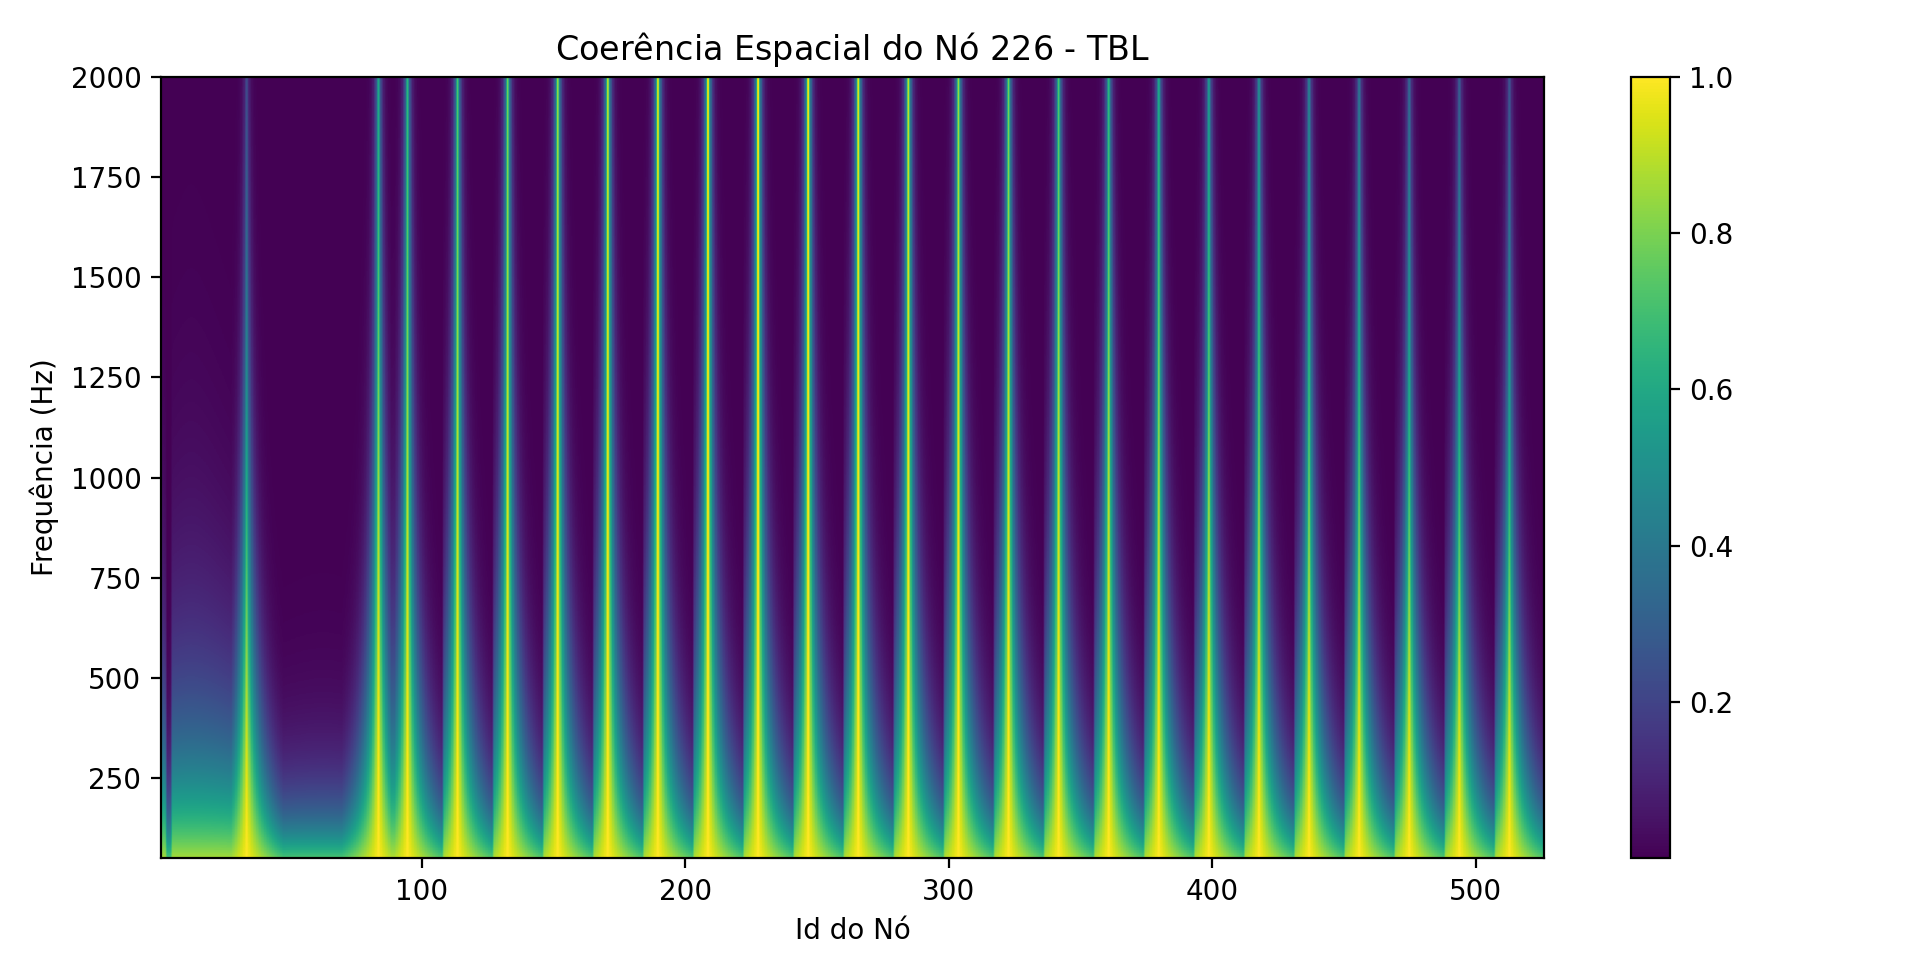
\includegraphics[width=0.9\columnwidth]{figures/coer_TBL.png}
	\caption{}
	\label{fig:coerTBL}
\end{figure}
O artigo de Marchetto~\cite{marchettoVibroacousticResponsePanels2017} que analisa o efeito de um campo acústico difuso sobre uma placa define o espectro cruzado da pressão do campo acústico como:

\begin{equation}
	S_{pp}(r,\omega) = S_{pp}(\omega) \frac{sin(k_0r)}{k_0r},
\end{equation}
onde $S_{pp}(\omega)$ é o auto espectro da pressão. Logo o termo representando a coerência espacial em função da frequência é $\Gamma(r,\omega) = \frac{sin(k_0r)}{k_0r}$, sendo $r = |x_\mu - x_v| = |(\xi_1,\xi_3)|$. A coerência do campo difuso pode ser observada na Figura~\ref{fig:coerDAF}.

\begin{figure}[H]
	\centering
	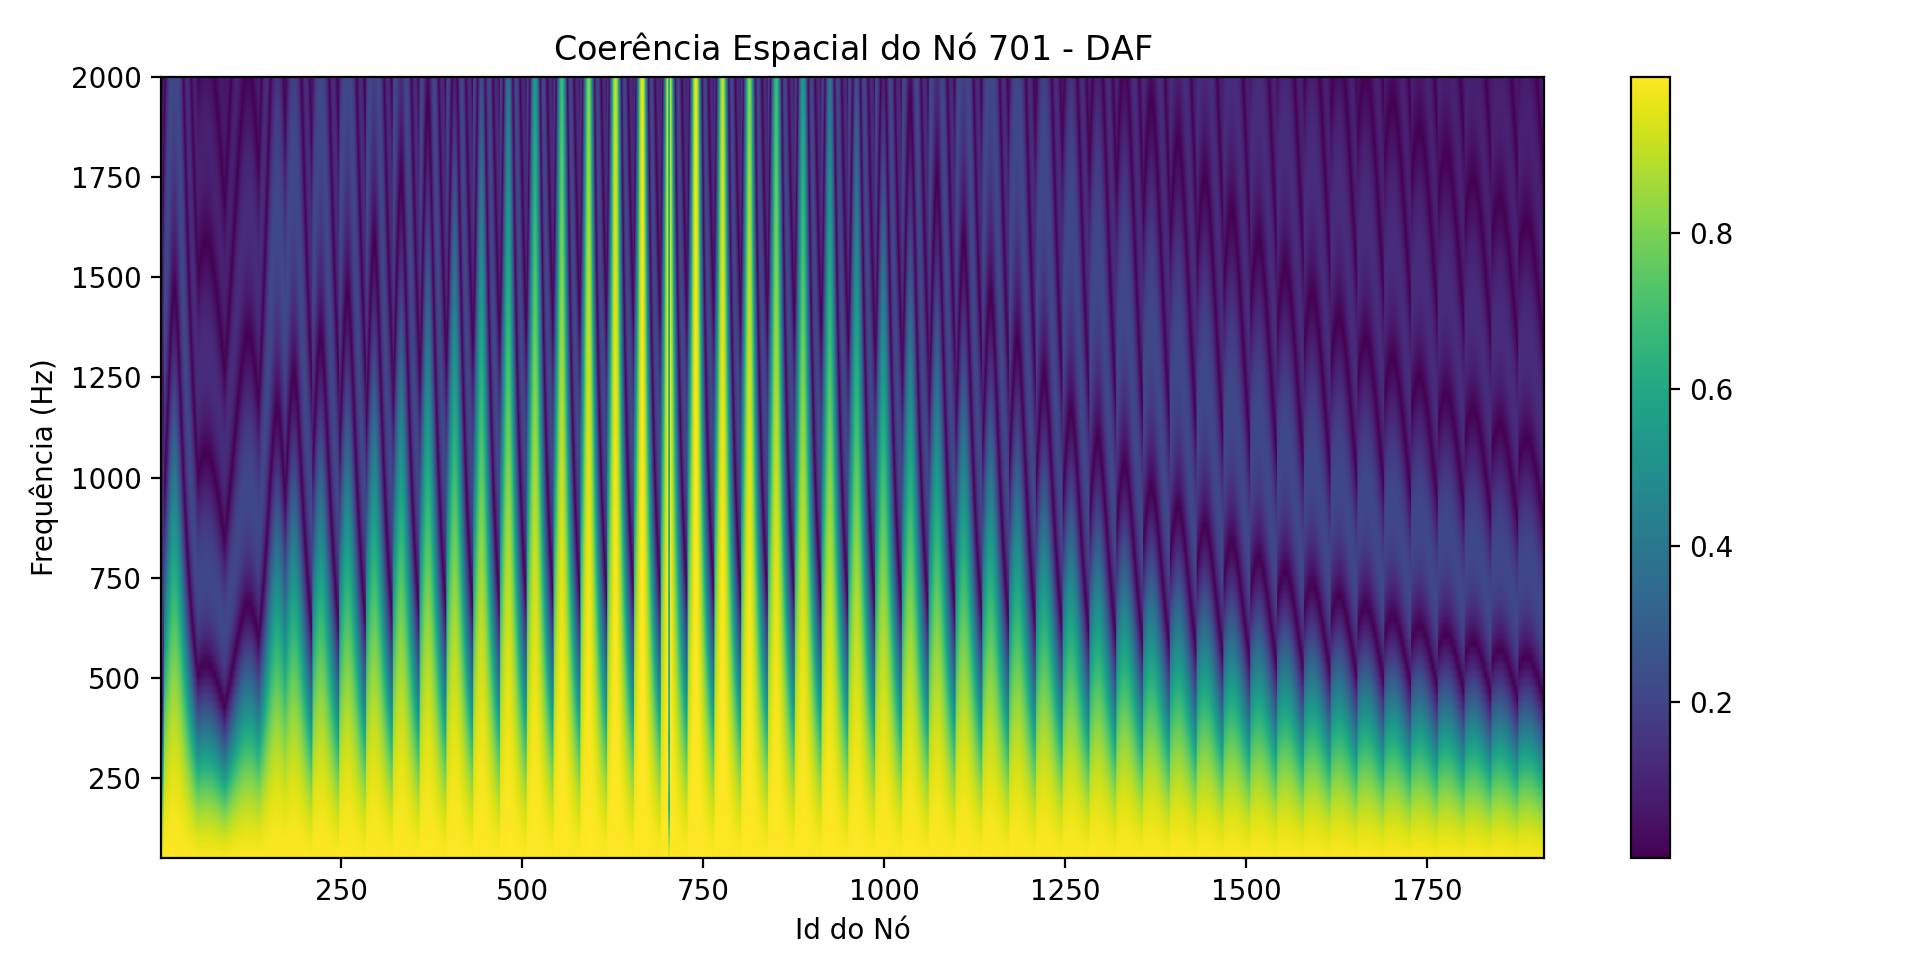
\includegraphics[width=0.9\columnwidth]{figures/coer_DAF.png}
	\caption{}
	\label{fig:coerDAF}
\end{figure}
\vfill
\subsection{Espectro Cruzado da Entrada}
Definindo-se o Espectro Cruzado da pressão como: 
\begin{equation}
	G_{x_\mu x_v}(\omega)=A_{x_\mu}\phi_{pp}(\omega)A_{x_v}\Gamma(\xi_1,\xi_3,\omega)
\end{equation}
Temos então as Figuras~\ref{fig:csdTBL} e \ref{fig:csdDAF}.

\begin{figure}[H]
	\centering
	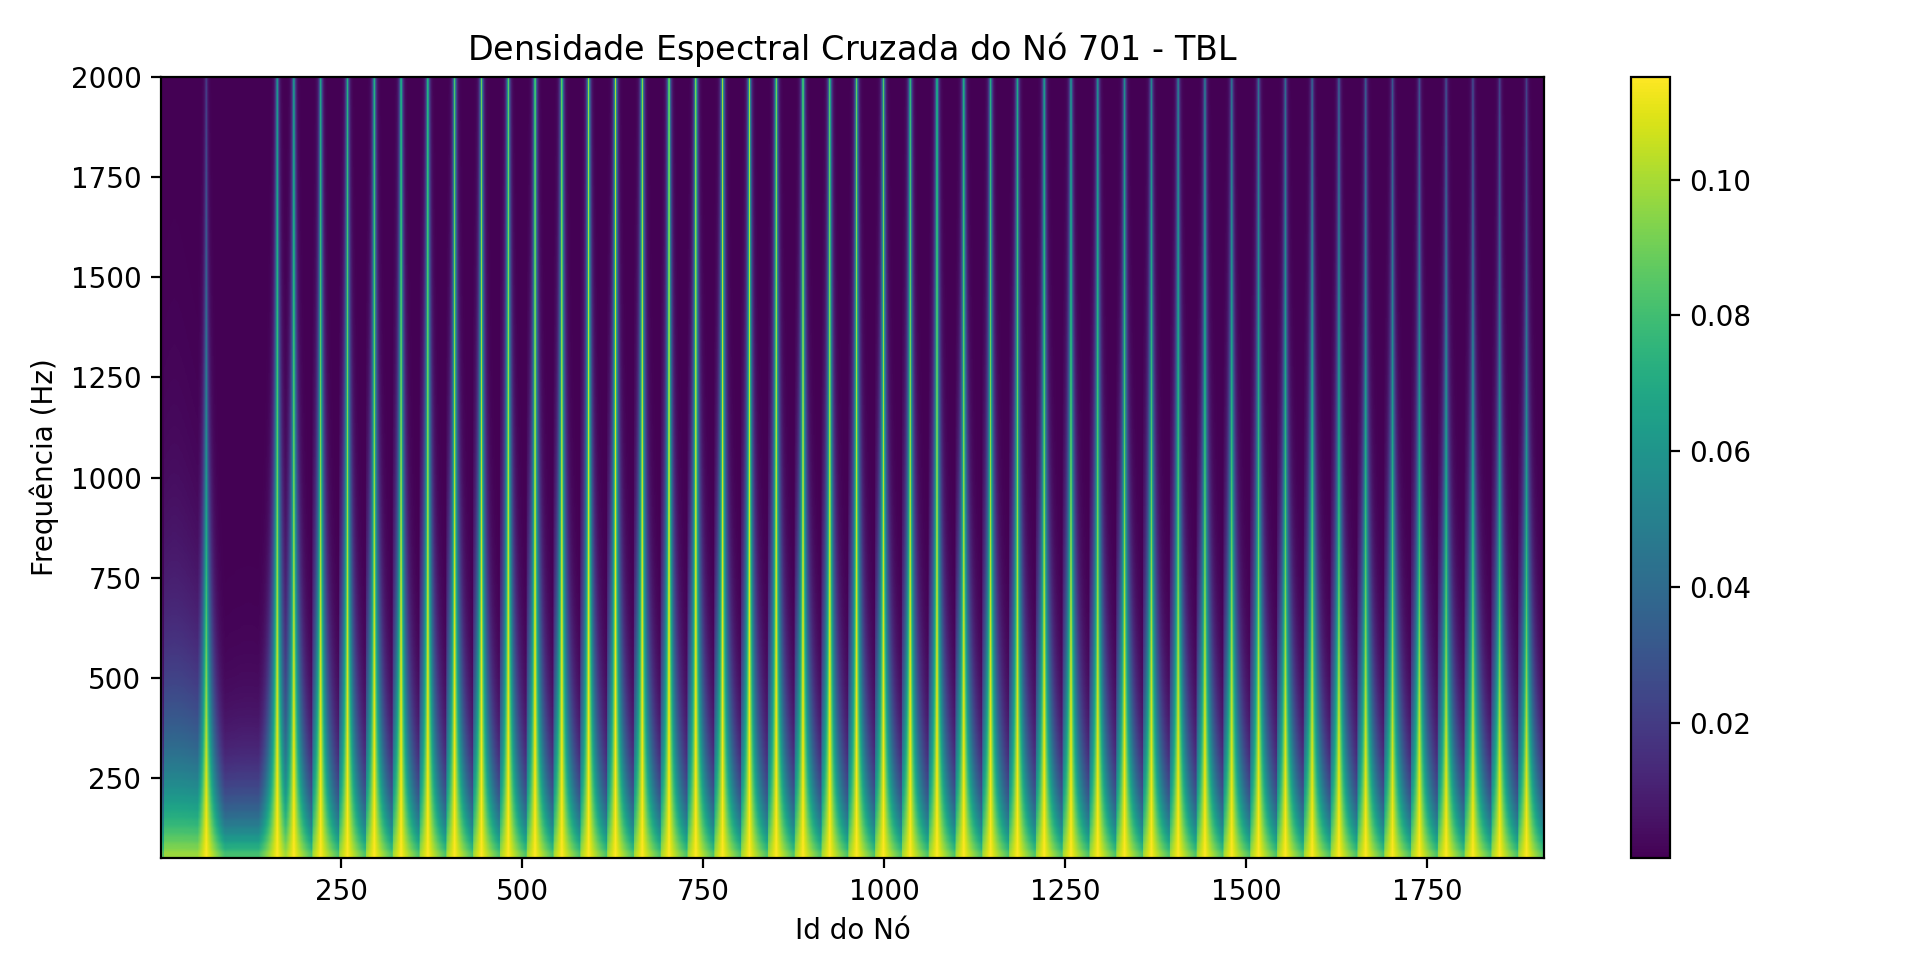
\includegraphics[width=0.9\columnwidth]{figures/csd_TBL.png}
	\caption{}
	\label{fig:csdTBL}
\end{figure}
Torna-se evidente a diferença entre a densidade espectral cruzada entre os casos de TBL e DAF e espera-se uma considerável diferença nas respostas calculadas para ambos os casos.
\begin{figure}[H]
	\centering
	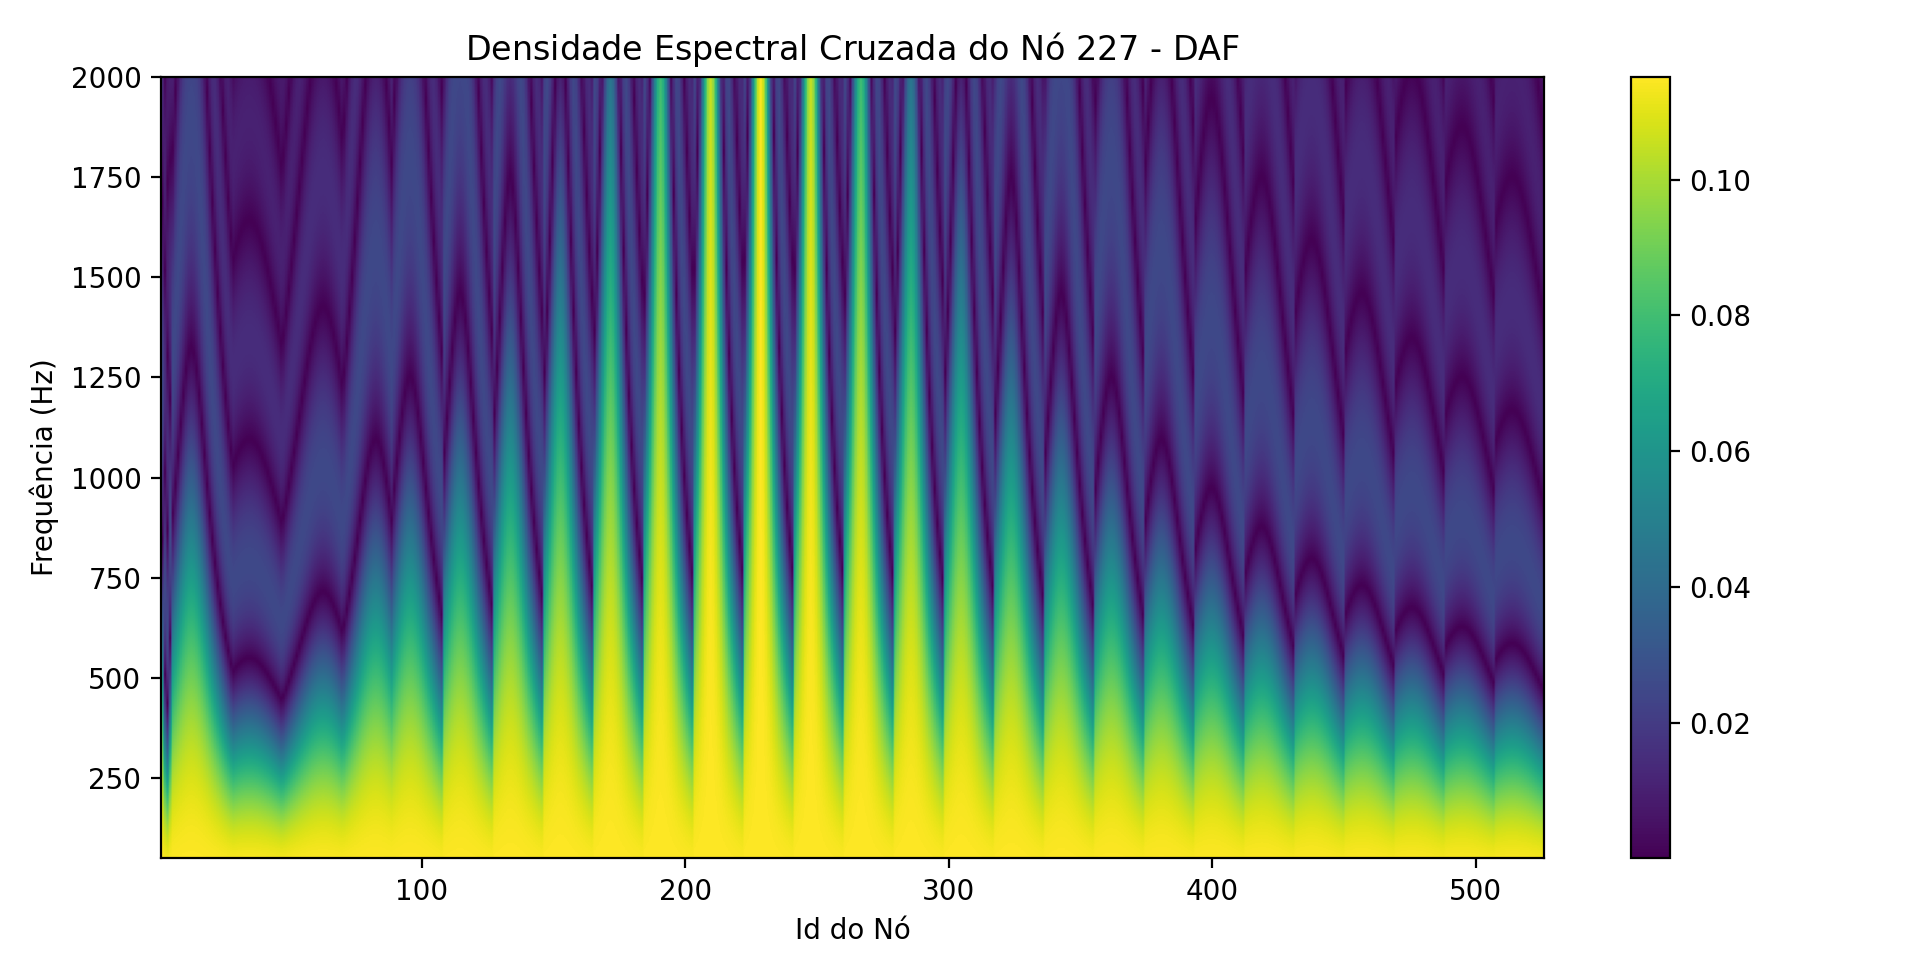
\includegraphics[width=0.9\columnwidth]{figures/csd_DAF.png}
	\caption{}
	\label{fig:csdDAF}
\end{figure}

\subsection{Função Resposta em Frequência}
Para encontrarmos as respostas a partir da entrada em pressão  deve-se deterinar as FRFs em relação ao ponto deobservação no nó 227.

\begin{equation}
	H_v = \frac{-j\omega}{\omega_n^2-\omega^2+j\eta\omega_n^2}
\end{equation}
\begin{figure}[H]
	\centering
	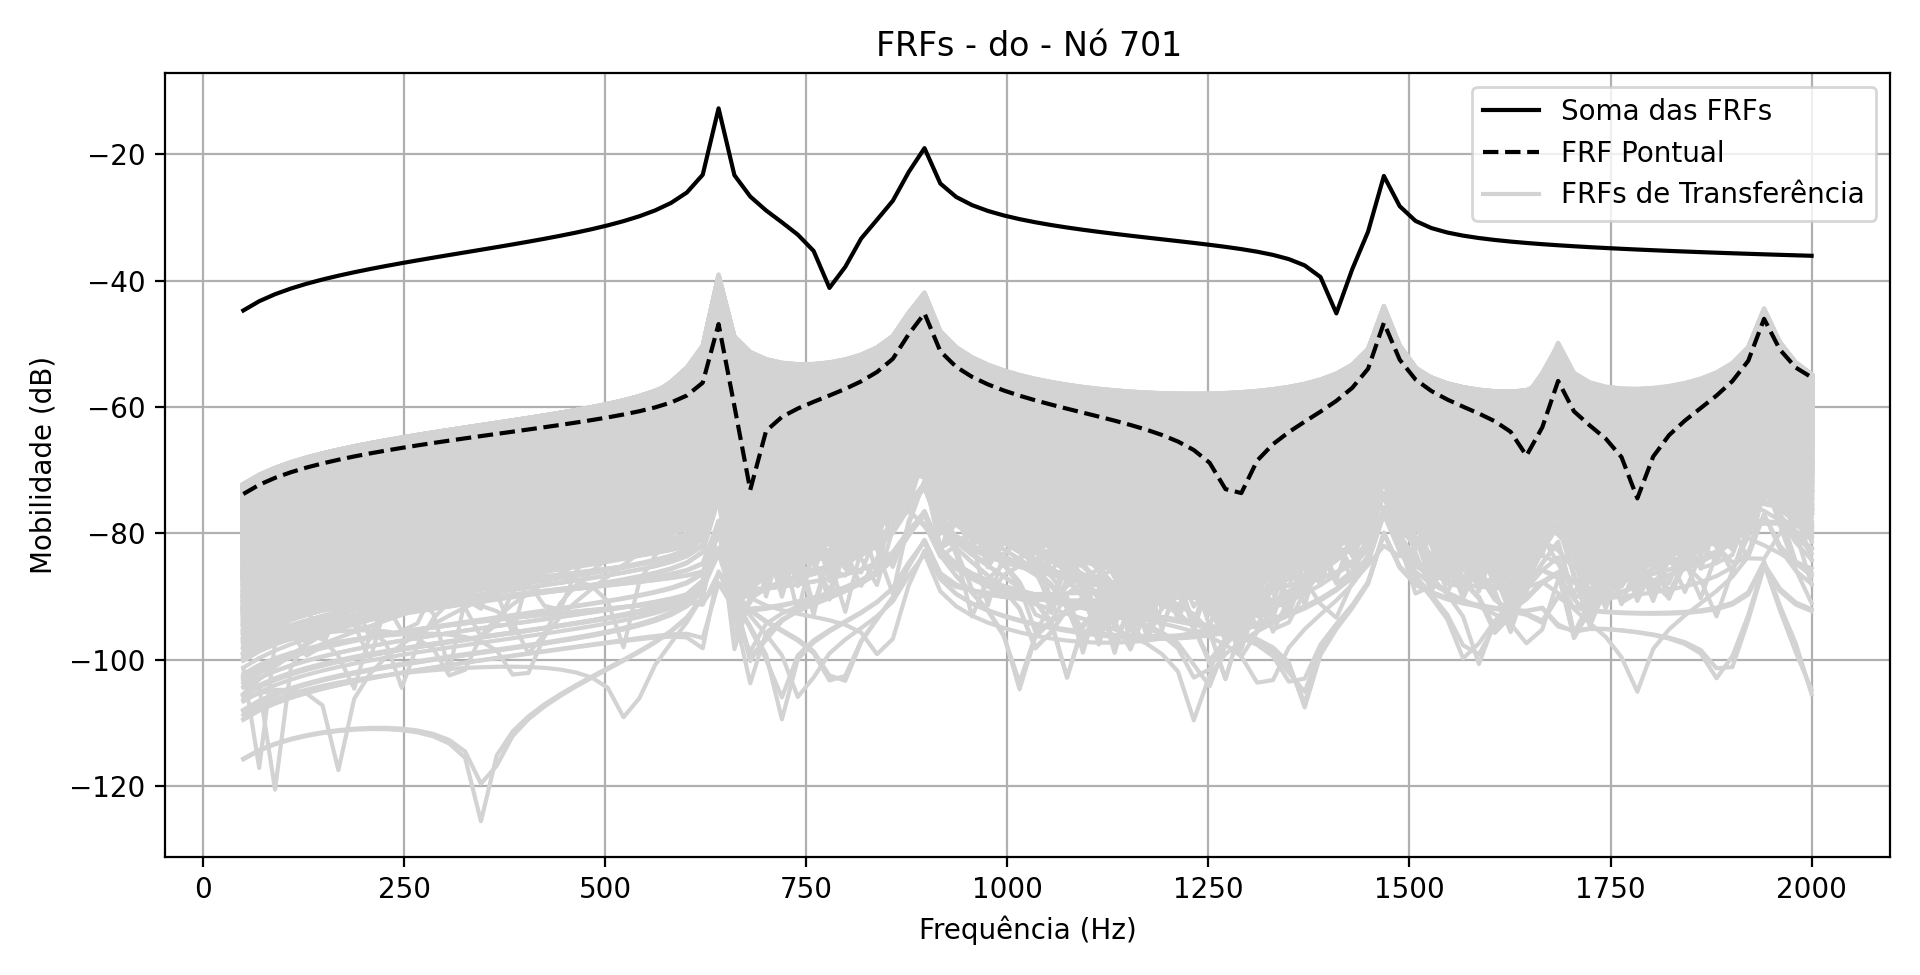
\includegraphics[width=0.9\columnwidth]{figures/frfs.png}
	\caption{Mobilidade}
	\label{fig:frf}
\end{figure}

\begin{figure}[H]
	\centering
	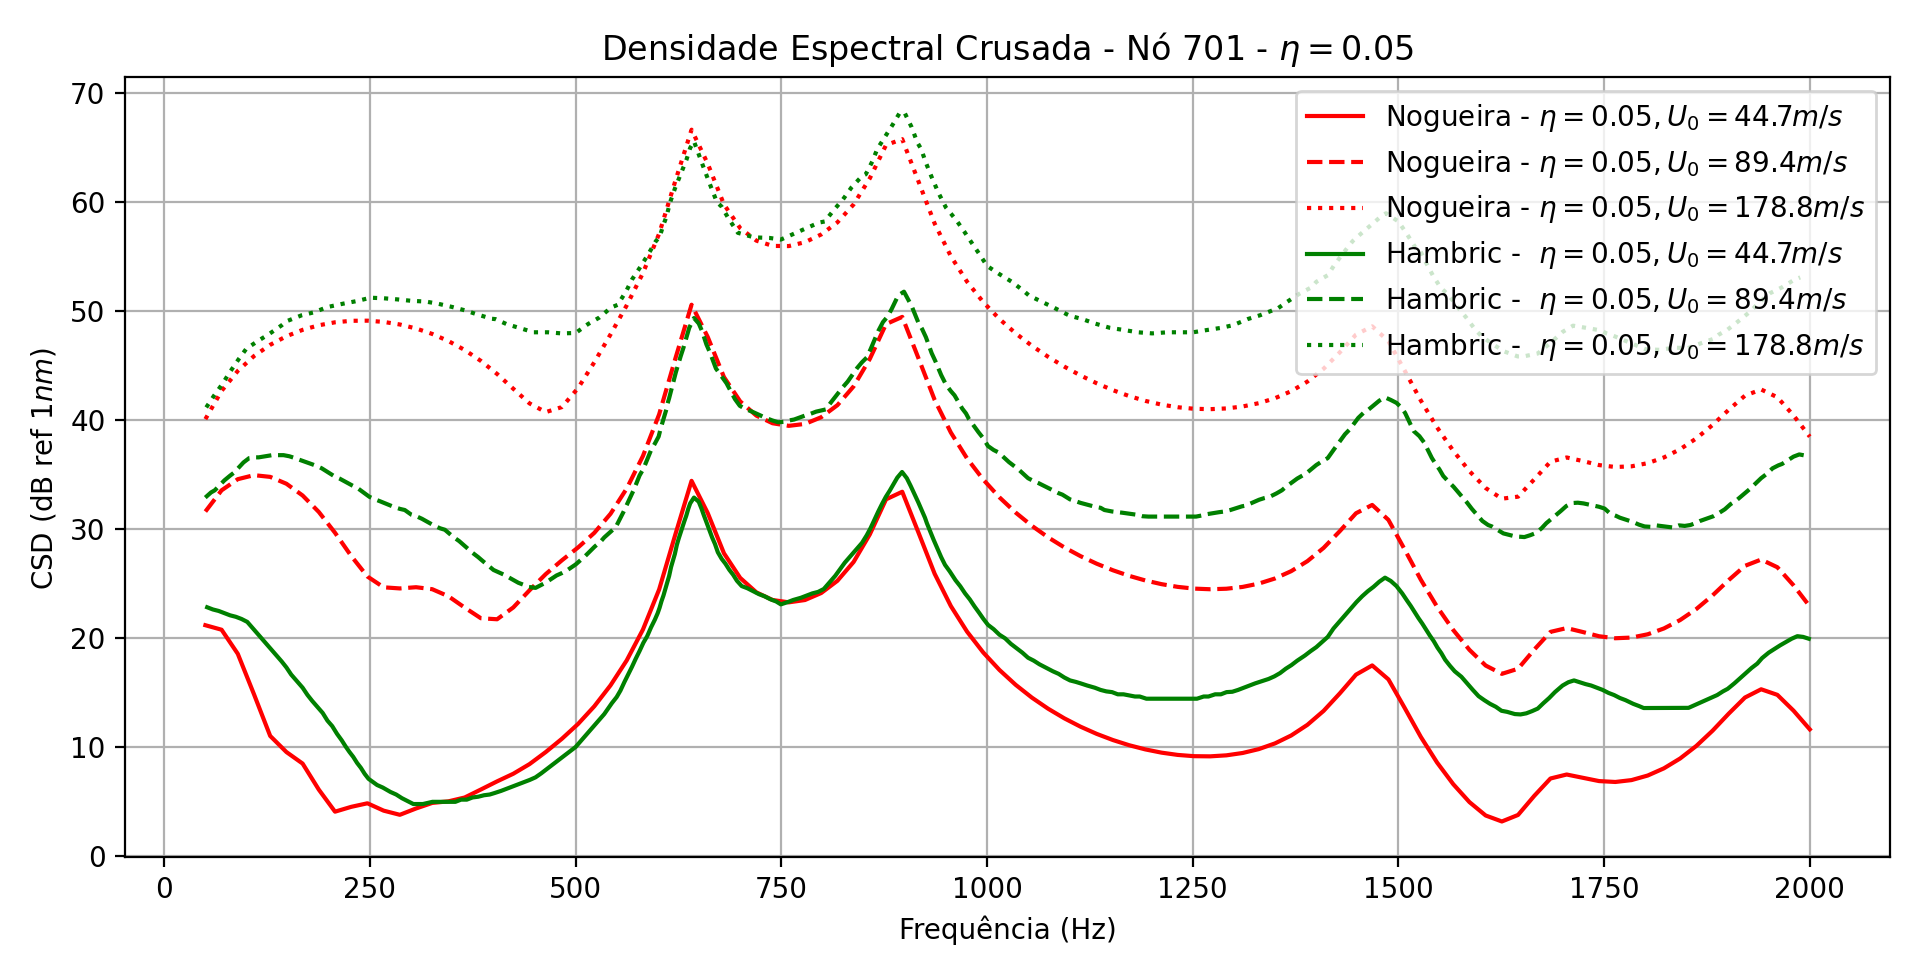
\includegraphics[width=0.9\columnwidth]{figures/csd_comp.png}
	\caption{}
	\label{fig:comp}
\end{figure}



\begin{equation}
	G_{uu}(y_i,y_j,\omega)\cong\sum_{\mu=1}^N\sum_{v=1}^NH_{u,F}^*(y_i/x_\mu,\omega)A_{x_\mu}\Phi_{pp}(x_\mu,x_v,\omega)A_{x_v}H_{u,F}(y_j/x_v,\omega)
\end{equation}

\begin{equation}
	\mathbf{G}_{yy}=\mathbf{H}_{xy}^{*T}\mathbf{G}_{xx}\mathbf{H}_{xy}
\end{equation}


\begin{figure}[H]
	\centering
	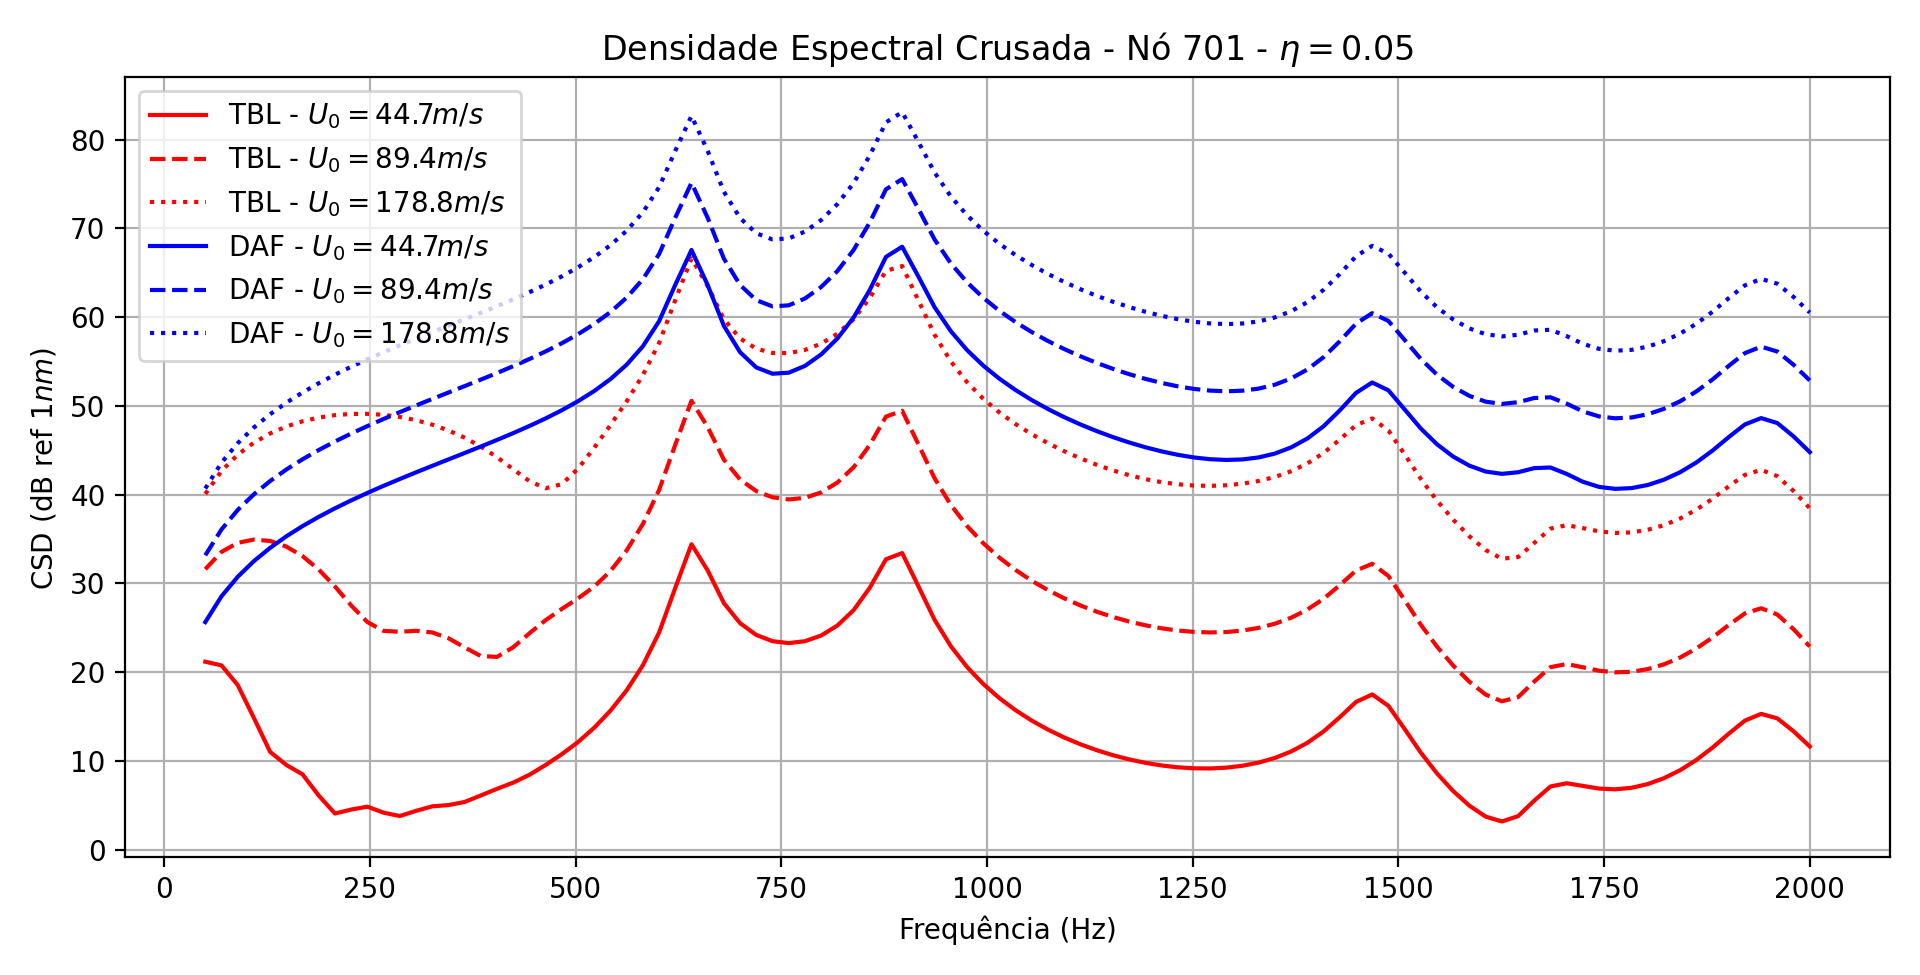
\includegraphics[width=0.9\columnwidth]{figures/csd_vel.png}
	\caption{}
	\label{fig:csdvel}
\end{figure}

\begin{figure}[H]
	\centering
	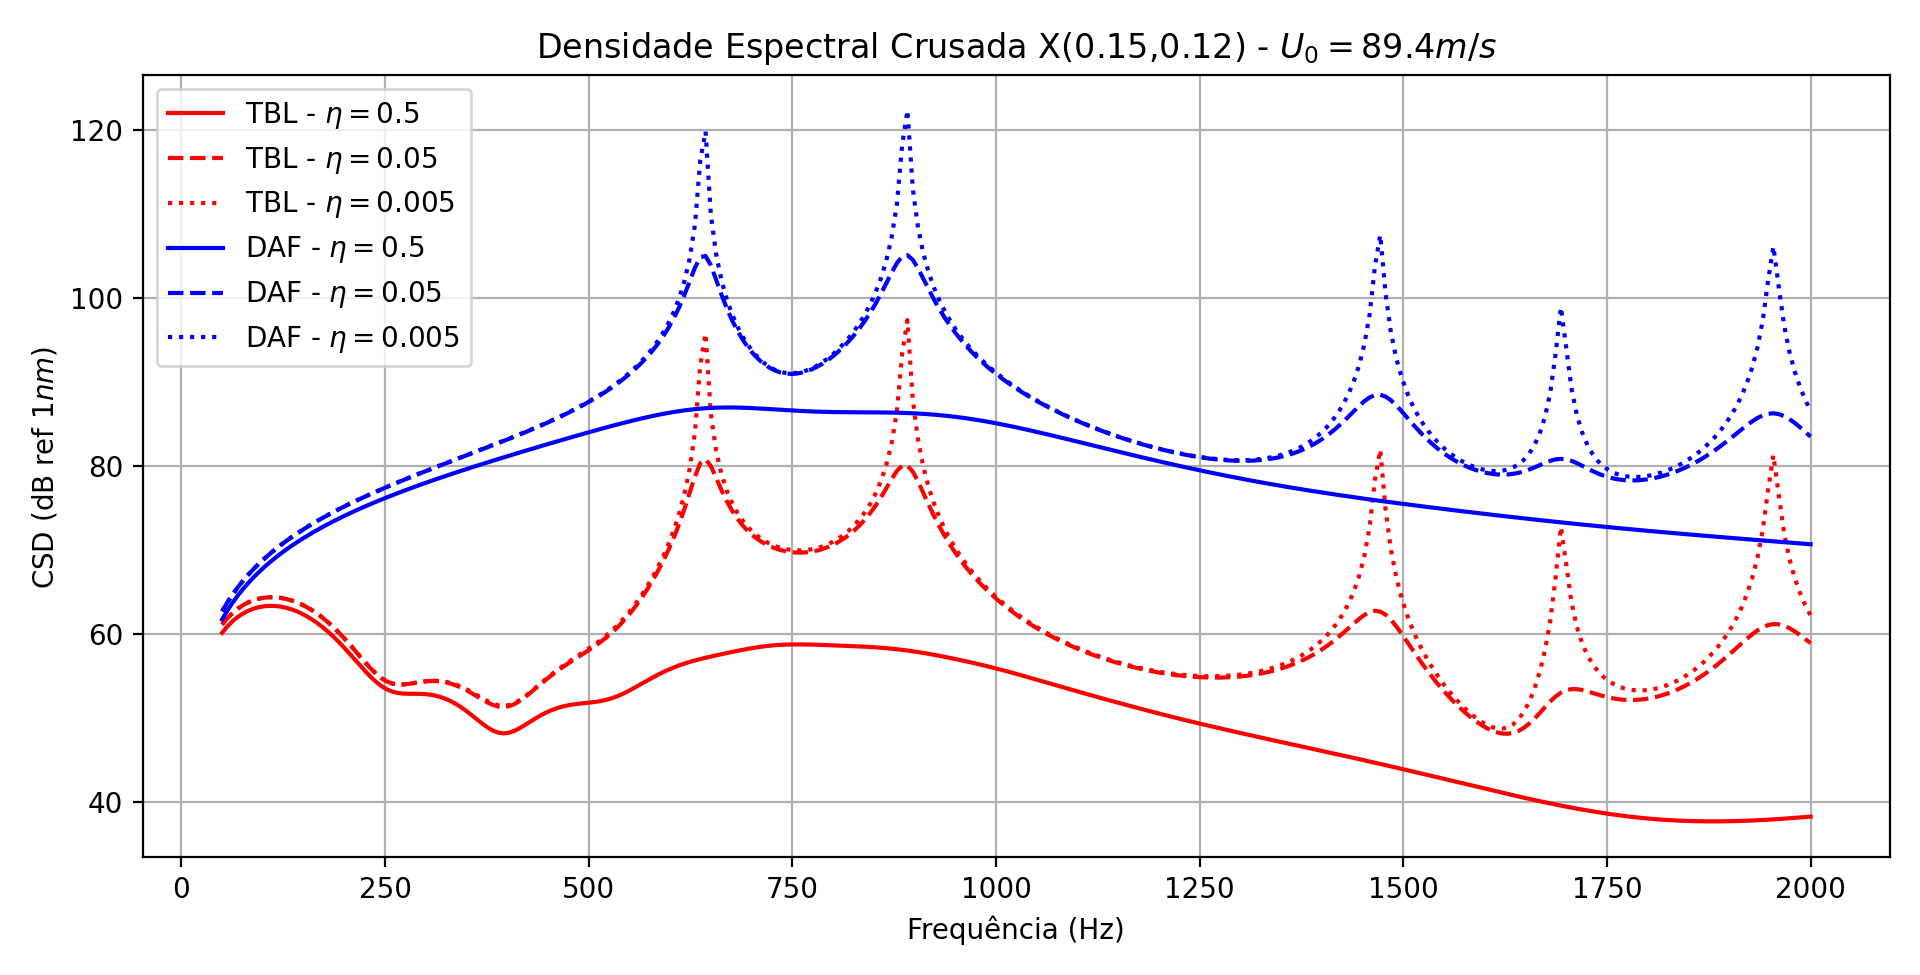
\includegraphics[width=0.9\columnwidth]{figures/csd_eta.png}
	\caption{}
	\label{fig:csdeta}
\end{figure}


%----------------------------------------------------------

\printbibliography

%----------------------------------------------------------

\end{document}